\section{Appendices}\label{sec:app:app}

\subsection{Description of simulation, synthesis and hardware tests}\label{sec:app:app_e}

Workflow for simulation and synthesis of firmware is described in \href{\gitbranch/README.md}{\texttt{README}} file.\\\\
List of useful TDF routines and commands for hardware tests:
\begin{itemize}
\item Check crate status\\
\greybox{\$ tdf run crate\_status}
\item Enable TTC signals on AMC13 for all MP7 modules\\
\greybox{\$ tdf run ttc\_enable}
\item Check lock of BC0 and LHC clock\\
\greybox{\$ tdf unittest <module> default}
\item Reset module\\
\greybox{\$ tdf mp7butler reset <module> --clksrc external --clkcfg default-ext}
\item Load firmware to scansd card on all MP7 modules [and load it into FPGAs]\\
\greybox{\$ tdf run uploadfw\_gt <tar file path> [--rebootfpga]}
\item Load firmware from scansd card into FPGAs\\
\greybox{\$ tdf run loadfw\_gt <fw build nr> <nr modules>}
\item Compare hardware results with test vector pattern (for a certain firmware build)\\
\greybox{\$ tdf run multiboard\_function\_test -h}
\item Setup links (GTHs)\\
\greybox{\$ tdf mp7butler rxmgts <module> -e <links>}
\item Align links (GTHs)\\
\greybox{\$ tdf mp7butler rxalign <module> -e <links> [--to-bx <alignment point>]}
\item Check minipods\\
\greybox{\$ tdf mp7butler minipods <module>}
\item ... (other routines are available in /nfshome0/ugtdev/software/tdf/etc/routines)
\end{itemize}

\subsubsection{Handling of timing errors in synthesis}\label{sec:app:synth_timing_errors}

Sometimes synthesis finish with timing errors on modules and no bit files are generated for those modules.
Most of the time the errors are low or not relevant and can be ignored. In this case generation
of a bit file could be done on the platform of synthesis with the following command in an environment where
vivado is running (see \href{\gitbranch/README.md}{\texttt{README}}):\\
\begin{itemize}
\item Generate bit file\\
\greybox{\$ vivado -mode batch -source <local path to mp7\_ugt\_legacy>/}\\
\greybox{scripts/vivado\_write\_bitstream.tcl -tclargs}\\
\greybox{<path to synth dir> <module number>}
\end{itemize}

\clearpage

\subsection{Configuration of GTHs}\label{sec:app:app_a}

The FPGA on MP7 board receives and transmits data via GTH transceivers.\\

\subsubsection{ZDC 5G scheme}\label{sec:app:zdc_5g_scheme}

ZDC data are provided on a 5 GHz link.
Figure~\ref{fig:app:zdc_5G_scheme} shows ZDC 5G link connection to \ugt system. (Currently only MP7 in slot 1 has a connection with ZDC.)\\

\begin{figure}[htb]
\centering
\includegraphics[width=15cm]{figures/zdc_5G_scheme}
\caption{ZDC 5G link connection}
\label{fig:app:zdc_5G_scheme}
\end{figure}

\clearpage

\subsubsection{GTH input connections}\label{sec:app:gth_i_conn}

Table~\ref{tab:app:gth_i_conn} contains the GTH input connections from MP7 MTP48 front connectors\footnote{"ch." means "channel", "pp conn." means "optical patch panel connector number"}:

\begin{longtable}{|l|c|c|c|c|c|c|c|l|}
\caption{GTH input connections}
    \label{tab:app:gth_i_conn}\\
\hline
\textbf{MTP48}& \textbf{minipod}& \textbf{quad}& \textbf{GTH ch.}& \textbf{GTH}& \textbf{MP7 ch.} &\textbf{pp}& \textbf{lane}& \textbf{data}\\
\hline
\hline
\endhead
RX1/1  & rx3/0  & 118 & X1Y35 & 10G & 0x00 & 1  & 0  & muon\\\hline
RX1/2  & rx3/1  &     & X1Y34 & 10G & 0x02 & 2  & 1  & muon\\\hline
RX1/3  & rx3/2  &     & X1Y33 & 10G & 0x04 & 3  & 2  & muon\\\hline
RX1/4  & rx3/3  &     & X1Y32 & 10G & 0x06 & 4  & 3  & muon\\\hline
RX1/5  & rx3/4  & 117 & X1Y31 & 10G & 0x08 & 5  & 4  & eg\\\hline
RX1/6  & rx3/5  &     & X1Y30 & 10G & 0x0A & 6  & 5  & eg\\\hline
RX1/7  & rx3/6  &     & X1Y29 & 10G & 0x0C & 7  & 6  & jet\\\hline
RX1/8  & rx3/7  &     & X1Y28 & 10G & 0x0E & 8  & 7  & jet\\\hline
RX1/9  & rx3/8  & 116 & X1Y27 & 10G & 0x10 & 9  & 8  & tau\\\hline
RX1/10 & rx3/9  &     & X1Y26 & 10G & 0x12 & 10 & 9  & tau\\\hline
RX1/11 & rx3/10 &     & X1Y25 & 10G & 0x14 & 11 & 10 & esums\\\hline
RX1/12 & rx3/11 &     & X1Y24 & 10G & 0x16 & 12 & 11 & CICADA\\\hline
RX1/13 & rx4/0  & 115 & X1Y23 & 10G & 0x18 & 13 & 12 & external conditions\\\hline
RX1/14 & rx4/1  &     & X1Y22 & 10G & 0x1A & 14 & 13 & external conditions\\\hline
RX1/15 & rx4/2  &     & X1Y21 & 10G & 0x1C & 15 & 14 & external conditions\\\hline
RX1/16 & rx4/3  &     & X1Y20 & 10G & 0x1E & 16 & 15 & external conditions\\\hline
RX1/17 & rx4/4  & 114 & X1Y19 & 10G & 0x20 & 17 & 16 & free\\\hline
RX1/18 & rx4/5  &     & X1Y18 & 10G & 0x22 & 18 & 17 & free\\\hline
RX1/19 & rx4/6  &     & X1Y17 & 10G & 0x24 & 19 & 18 & free\\\hline
RX1/20 & rx4/7  &     & X1Y16 & 10G & 0x26 & 20 & 19 & free\\\hline
RX1/21 & rx4/8  & 113 & X1Y15 & 10G & 0x28 & 21 & 20 & free\\\hline
RX1/22 & rx4/9  &     & X1Y14 & 10G & 0x2A & 22 & 21 & free\\\hline
RX1/23 & rx4/10 &     & X1Y13 & 10G & 0x2C & 23 & 22 & free\\\hline
RX1/24 & rx4/11 &     & X1Y12 & 10G & 0x2E & 24 & 23 & free\\\hline
RX1/25 & rx5/0  & 112 & X1Y11 & 10G & 0x30 & nc & 24 & -\\\hline
RX1/28 & rx5/3  &     & X1Y10 & 10G & 0x32 & nc & 25 & -\\\hline
RX1/26 & rx5/1  &     & X1Y09 & 10G & 0x34 & nc & 26 & -\\\hline
RX1/27 & rx5/2  &     & X1Y08 & 10G & 0x36 & nc & 27 & -\\\hline
RX1/30 & rx5/5  & 111 & X1Y07 &  x  & 0x38 & nc & 28 & -\\\hline
RX1/29 & rx5/4  &     & X1Y06 &  x  & 0x3A & nc & 29 & -\\\hline
RX1/31 & rx5/6  &     & X1Y05 &  x  & 0x3C & nc & 30 & -\\\hline
RX1/32 & rx5/7  &     & X1Y04 &  x  & 0x3E & nc & 31 & -\\\hline
RX1/33 & rx5/8  & 110 & X1Y03 &  x  & 0x40 & nc & 32 & -\\\hline
RX1/34 & rx5/9  &     & X1Y02 &  x  & 0x42 & nc & 33 & -\\\hline
RX1/35 & rx5/10 &     & X1Y01 &  x  & 0x44 & nc & 34 & -\\\hline
RX1/36 & rx5/11 &     & X1Y00 &  x  & 0x46 & nc & 35 & -\\\hline
RX2/26 & rx2/1  & 210 & X0Y00 &  x  & 0x48 & nc & 36 & -\\\hline        
RX2/25 & rx2/0  &     & X0Y01 &  x  & 0x4A & nc & 37 & -\\\hline        
RX2/28 & rx2/3  &     & X0Y02 &  x  & 0x4C & nc & 38 & -\\\hline        
RX2/27 & rx2/2  &     & X0Y03 &  x  & 0x4E & nc & 39 & -\\\hline   
RX2/30 & rx2/5  & 211 & X0Y04 &  x  & 0x50 & nc & 40 & -\\\hline   
RX2/29 & rx2/4  &     & X0Y05 &  x  & 0x52 & nc & 41 & -\\\hline   
RX2/31 & rx2/7  &     & X0Y06 &  x  & 0x54 & nc & 42 & -\\\hline   
RX2/32 & rx2/6  &     & X0Y07 &  x  & 0x56 & nc & 43 & -\\\hline   
RX2/33 & rx2/8  & 212 & X0Y08 &  x  & 0x58 & nc & 44 & -\\\hline   
RX2/35 & rx2/10 &     & X0Y09 &  x  & 0x5A & nc & 45 & -\\\hline   
RX2/34 & rx2/9  &     & X0Y10 &  x  & 0x5C & nc & 46 & -\\\hline   
RX2/36 & rx2/11 &     & X0Y11 &  x  & 0x5E & nc & 47 & -\\\hline   
RX2/14 & rx1/1  & 213 & X0Y12 &  x  & 0x60 & nc & 48 & -\\\hline   
RX2/13 & rx1/0  &     & X0Y13 &  x  & 0x62 & nc & 49 & -\\\hline   
RX2/16 & rx1/3  &     & X0Y14 &  x  & 0x64 & nc & 50 & -\\\hline   
RX2/15 & rx1/2  &     & X0Y15 &  x  & 0x66 & nc & 51 & -\\\hline   
RX2/18 & rx1/5  & 214 & X0Y16 &  x  & 0x68 & nc & 52 & -\\\hline   
RX2/17 & rx1/4  &     & X0Y17 &  x  & 0x6A & nc & 53 & -\\\hline   
RX2/20 & rx1/7  &     & X0Y18 &  x  & 0x6C & nc & 54 & -\\\hline   
RX2/19 & rx1/6  &     & X0Y19 &  x  & 0x6E & nc & 55 & -\\\hline   
RX2/22 & rx1/9  & 215 & X0Y20 &  x  & 0x70 & nc & 56 & -\\\hline   
RX2/21 & rx1/8  &     & X0Y21 &  x  & 0x72 & nc & 57 & -\\\hline   
RX2/23 & rx1/10 &     & X0Y22 &  x  & 0x74 & nc & 58 & -\\\hline   
RX2/24 & rx1/11 &     & X0Y23 &  x  & 0x76 & nc & 59 & -\\\hline   
RX2/2  & rx0/1  & 216 & X0Y24 &  x  & 0x78 & nc & 60 & -\\\hline   
RX2/1  & rx0/0  &     & X0Y25 &  x  & 0x7A & nc & 61 & -\\\hline   
RX2/4  & rx0/3  &     & X0Y26 &  x  & 0x7C & nc & 62 & -\\\hline   
RX2/3  & rx0/2  &     & X0Y27 &  x  & 0x7E & nc & 63 & -\\\hline   
RX2/6  & rx0/5  & 217 & X0Y28 &  x  & 0x80 & nc & 64 & -\\\hline   
RX2/5  & rx0/4  &     & X0Y29 &  x  & 0x82 & nc & 65 & -\\\hline   
RX2/8  & rx0/7  &     & X0Y30 &  x  & 0x84 & nc & 66 & -\\\hline   
RX2/7  & rx0/6  &     & X0Y31 &  x  & 0x86 & nc & 67 & -\\\hline   
RX2/10 & rx0/9  & 218 & X0Y32 &  5G & 0x88 & nc & 68 & -\\\hline   
RX2/9  & rx0/8  &     & X0Y33 &  5G & 0x8A & nc & 69 & -\\\hline   
RX2/11 & rx0/10 &     & X0Y34 &  5G & 0x8C & nc & 70 & -\\\hline   
RX2/12 & rx0/11 &     & X0Y35 &  5G & 0x8E & nc & 71 & ZDC\\\hline   
\end{longtable}                  

\clearpage

\subsubsection{GTH output connections}\label{sec:app:gth_o_conn}

Table~\ref{tab:app:gth_o_conn} contains the GTH output connections to MP7 MTP front connectors:

\begin{longtable}{|l|c|c|c|c|c|c|c|l|}
\caption{GTH output connections}
    \label{tab:app:gth_o_conn}\\
\hline
\textbf{MTP48}& \textbf{minipod}& \textbf{quad}& \textbf{GTH ch.}& \textbf{GTH}& \textbf{MP7 ch.} &\textbf{pp}& \textbf{lane}& \textbf{data}\\
\hline
\hline
\endhead
TX1/1  & tx3/0  & 118 & X1Y35 & 10G & 0x01 & nc & 0  & -\\\hline
TX1/2  & tx3/1  &     & X1Y34 & 10G & 0x03 & nc & 1  & -\\\hline
TX1/3  & tx3/2  &     & X1Y33 & 10G & 0x05 & nc & 2  & -\\\hline
TX1/4  & tx3/3  &     & X1Y32 & 10G & 0x07 & nc & 3  & -\\\hline
TX1/5  & tx3/4  & 117 & X1Y31 & 10G & 0x09 & nc & 4  & -\\\hline
TX1/6  & tx3/5  &     & X1Y30 & 10G & 0x0b & nc & 5  & -\\\hline
TX1/7  & tx3/6  &     & X1Y29 & 10G & 0x0d & nc & 6  & -\\\hline
TX1/8  & tx3/7  &     & X1Y28 & 10G & 0x0f & nc & 7  & -\\\hline
TX1/9  & tx3/8  & 116 & X1Y27 & 10G & 0x11 & nc & 8  & -\\\hline
TX1/10 & tx3/9  &     & X1Y26 & 10G & 0x13 & nc & 9  & -\\\hline
TX1/11 & tx3/10 &     & X1Y25 & 10G & 0x15 & nc & 10 & -\\\hline
TX1/12 & tx3/11 &     & X1Y24 & 10G & 0x17 & nc & 11 & -\\\hline
TX1/13 & tx4/0  & 115 & X1Y23 & 10G & 0x19 & nc & 12 & -\\\hline
TX1/14 & tx4/1  &     & X1Y22 & 10G & 0x1b & nc & 13 & -\\\hline
TX1/15 & tx4/2  &     & X1Y21 & 10G & 0x1d & nc & 14 & -\\\hline
TX1/16 & tx4/3  &     & X1Y20 & 10G & 0x1f & nc & 15 & -\\\hline
TX1/17 & tx4/4  & 114 & X1Y19 & 10G & 0x21 & nc & 16 & readout (AMC13)\\\hline
TX1/18 & tx4/5  &     & X1Y18 & 10G & 0x23 & nc & 17 & readout (AMC13)\\\hline
TX1/19 & tx4/6  &     & X1Y17 & 10G & 0x25 & nc & 18 & readout (AMC13)\\\hline
TX1/20 & tx4/7  &     & X1Y16 & 10G & 0x27 & nc & 19 & readout (AMC13)\\\hline
TX1/21 & tx4/8  & 113 & X1Y15 & 10G & 0x29 & nc & 20 & readout (AMC13)\\\hline
TX1/22 & tx4/9  &     & X1Y14 & 10G & 0x2b & nc & 21 & readout (AMC13)\\\hline
TX1/23 & tx4/10 &     & X1Y13 & 10G & 0x2d & nc & 22 & readout (AMC13)\\\hline
TX1/24 & tx4/11 &     & X1Y12 & 10G & 0x2f & nc & 23 & readout (AMC13)\\\hline
TX1/25 & tx5/0  & 112 & X1Y11 & 10G & 0x31 & nc & 24 & readout (AMC13)\\\hline
TX1/26 & tx5/1  &     & X1Y10 & 10G & 0x33 & nc & 25 & readout (AMC13)\\\hline
TX1/27 & tx5/2  &     & X1Y09 & 10G & 0x35 & nc & 26 & -\\\hline
TX1/28 & tx5/3  &     & X1Y08 & 10G & 0x37 & nc & 27 & -\\\hline
TX1/29 & tx5/4  & 111 & X1Y07 & 10G & 0x39 & nc & 28 & scouting\\\hline
TX1/30 & tx5/5  &     & X1Y06 & 10G & 0x3b & nc & 29 & scouting\\\hline
TX1/31 & tx5/6  &     & X1Y05 & 10G & 0x3d & nc & 30 & scouting\\\hline
TX1/32 & tx5/7  &     & X1Y04 & 10G & 0x3f & nc & 31 & scouting\\\hline
TX1/33 & tx5/8  & 110 & X1Y03 &  x  & 0x41 & nc & 32 & -\\\hline
TX1/34 & tx5/9  &     & X1Y02 &  x  & 0x43 & nc & 33 & -\\\hline
TX1/35 & tx5/10 &     & X1Y01 &  x  & 0x45 & nc & 34 & -\\\hline
TX1/36 & tx5/11 &     & X1Y00 &  x  & 0x47 & nc & 35 & -\\\hline
TX2/26 & tx2/1  & 210 & X0Y00 &  x  & 0x49 & nc & 36 & -\\\hline
TX2/25 & tx2/0  &     & X0Y01 &  x  & 0x4b & nc & 37 & -\\\hline
TX2/28 & tx2/3  &     & X0Y02 &  x  & 0x4d & nc & 38 & -\\\hline
TX2/27 & tx2/2  &     & X0Y03 &  x  & 0x4f & nc & 39 & -\\\hline
TX2/30 & tx2/5  & 211 & X0Y04 &  x  & 0x51 & nc & 40 & -\\\hline
TX2/29 & tx2/4  &     & X0Y05 &  x  & 0x53 & nc & 41 & -\\\hline
TX2/32 & tx2/7  &     & X0Y06 &  x  & 0x55 & nc & 42 & -\\\hline
TX2/31 & tx2/6  &     & X0Y07 &  x  & 0x57 & nc & 43 & -\\\hline
TX2/34 & tx2/8  & 212 & X0Y08 &  x  & 0x59 & nc & 44 & -\\\hline
TX2/33 & tx2/10 &     & X0Y09 &  x  & 0x5b & nc & 45 & -\\\hline
TX2/35 & tx2/9  &     & X0Y10 &  x  & 0x5d & nc & 46 & -\\\hline
TX2/36 & tx2/11 &     & X0Y11 &  x  & 0x5f & nc & 47 & -\\\hline
TX2/14 & tx1/1  & 213 & X0Y12 &  x  & 0x61 & nc & 48 & -\\\hline
TX2/13 & tx1/0  &     & X0Y13 &  x  & 0x63 & nc & 49 & -\\\hline
TX2/16 & tx1/3  &     & X0Y14 &  x  & 0x65 & nc & 50 & -\\\hline
TX2/15 & tx1/2  &     & X0Y15 &  x  & 0x67 & nc & 51 & -\\\hline
TX2/18 & tx1/5  & 214 & X0Y16 &  x  & 0x69 & nc & 52 & -\\\hline
TX2/17 & tx1/4  &     & X0Y17 &  x  & 0x6b & nc & 53 & -\\\hline
TX2/20 & tx1/7  &     & X0Y18 &  x  & 0x6d & nc & 54 & -\\\hline
TX2/19 & tx1/6  &     & X0Y19 &  x  & 0x6f & nc & 55 & -\\\hline
TX2/22 & tx1/9  & 215 & X0Y20 &  x  & 0x71 & nc & 56 & -\\\hline
TX2/21 & tx1/8  &     & X0Y21 &  x  & 0x73 & nc & 57 & -\\\hline
TX2/23 & tx1/10 &     & X0Y22 &  x  & 0x75 & nc & 58 & -\\\hline
TX2/24 & tx1/11 &     & X0Y23 &  x  & 0x77 & nc & 59 & -\\\hline
TX2/2  & tx0/1  & 216 & X0Y24 &  x  & 0x79 & nc & 60 & -\\\hline
TX2/1  & tx0/0  &     & X0Y25 &  x  & 0x7b & nc & 61 & -\\\hline
TX2/4  & tx0/3  &     & X0Y26 &  x  & 0x7d & nc & 62 & -\\\hline
TX2/3  & tx0/2  &     & X0Y27 &  x  & 0x7f & nc & 63 & -\\\hline
TX2/6  & tx0/5  & 217 & X0Y28 &  x  & 0x81 & nc & 64 & -\\\hline
TX2/5  & tx0/4  &     & X0Y29 &  x  & 0x83 & nc & 65 & -\\\hline
TX2/8  & tx0/7  &     & X0Y30 &  x  & 0x85 & nc & 66 & -\\\hline
TX2/7  & tx0/6  &     & X0Y31 &  x  & 0x87 & nc & 67 & -\\\hline
TX2/10 & tx0/9  & 218 & X0Y32 &  x  & 0x89 & nc & 68 & -\\\hline
TX2/9  & tx0/8  &     & X0Y33 &  x  & 0x8b & nc & 69 & -\\\hline
TX2/11 & tx0/10 &     & X0Y34 &  x  & 0x8d & nc & 70 & -\\\hline
TX2/12 & tx0/11 &     & X0Y35 &  x  & 0x8f & nc & 71 & -\\\hline

\end{longtable}

\clearpage

\subsubsection{Data on GTHs}\label{sec:app:gth_conf_table}

In Table~\ref{tab:app:gth_conf} configuration of GTHs~\cite{GTHs} for Global Trigger is shown\footnote{"MGT" means "MGT\_BANK", "GTHE2" means "GTHE2\_CHANNEL", "RX" means "GTH receiver", "TX" means "GTH transmitter"}.

\begin{longtable}{|l|c|c|c|c|c|}
\caption{Configuration of GTHs}
    \label{tab:app:gth_conf}\\
\hline
\textbf{Objects}& \textbf{Link}& \textbf{MGT}& \textbf{GTHE2}& \textbf{RX}& \textbf{TX}\\
\hline
\hline
\endhead
MU0..MU1  & 0  & 118 & X1Y35 & x &   \\\hline
MU2..MU3  & 1  & 118 & X1Y34 & x &   \\\hline
MU4..MU5  & 2  & 118 & X1Y33 & x &   \\\hline
MU6..MU7  & 3  & 118 & X1Y32 & x &   \\\hline
EG0..EG5  & 4  & 117 & X1Y31 & x &   \\\hline
EG6..EG11 & 5  & 117 & X1Y30 & x &   \\\hline
JET0..JET5  & 6  & 117 & X1Y29 & x &   \\\hline
JET6..JET11 & 7  & 117 & X1Y28 & x &   \\\hline
TAU0..TAU5  & 8  & 116 & X1Y27 & x &   \\\hline
TAU6..TAU11 & 9  & 116 & X1Y26 & x &   \\\hline
ESUMS  & 10  & 116 & X1Y25 & x &   \\\hline
CICADA (BJET0..BJET5, ...)& 11  & 116 & X1Y24 & x &   \\\hline
EXT\_COND[0:63] & 12  & 115 & X1Y23 & x &   \\\hline
EXT\_COND[64:127] & 13  & 115 & X1Y22 & x &   \\\hline
EXT\_COND[128:191] & 14  & 115 & X1Y21 & x &   \\\hline
EXT\_COND[192:255] & 15  & 115 & X1Y20 & x &   \\\hline
free & 16  & 114 & X1Y19 & x &   \\\hline
free & 17  & 114 & X1Y18 & x &   \\\hline
free & 18  & 114 & X1Y17 & x &   \\\hline
free & 19  & 114 & X1Y16 & x &   \\\hline
free & 20  & 113 & X1Y15 & x &   \\\hline
free & 21  & 113 & X1Y14 & x &   \\\hline
free & 22  & 113 & X1Y13 & x &   \\\hline
free & 23  & 113 & X1Y12 & x &   \\\hline\hline
ALGO\_AFTER\_GTLOGIC[0:191] & 16  & 114 & X1Y19 &   & x \\\hline
ALGO\_AFTER\_GTLOGIC[192:383] & 17  & 114 & X1Y18 &   & x \\\hline
ALGO\_AFTER\_GTLOGIC[383:511] & 18  & 114 & X1Y17 &   & x \\\hline
ALGO\_AFTER\_BXMASK[0:191] & 19  & 114 & X1Y16 &   & x \\\hline
ALGO\_AFTER\_BXMASK[192:383] & 20  & 113 & X1Y15 &   & x \\\hline
ALGO\_AFTER\_BXMASK[383:511] & 21  & 113 & X1Y14 &   & x \\\hline
ALGO\_AFTER\_BXMASK[0:191] & 22  & 113 & X1Y13 &   & x \\\hline
ALGO\_AFTER\_BXMASK[192:383] & 23  & 113 & X1Y12 &   & x \\\hline
ALGO\_AFTER\_BXMASK[383:511] & 24  & 112 & X1Y11 &   & x \\\hline
Bunchcounters, ... & 25  & 112 & X1Y10 &   & x \\\hline
SCOUTING & 28  & 111 & X1Y07 &   & x \\\hline
SCOUTING & 29  & 111 & X1Y06 &   & x \\\hline
SCOUTING & 30  & 111 & X1Y05 &   & x \\\hline
SCOUTING & 31  & 111 & X1Y04 &   & x \\\hline\hline
ZDC & 71  & 218 & X0Y35 & x & \\\hline
\end{longtable}

\clearpage

\subsection{Configuration of optical input links}\label{sec:app:app_b}

% Figure~\ref{fig:app:ugt_inputs} shows the configuration of optical links to Global Trigger.\\
% Links 0..3 contains muon data from GMT, links 4..10 data from Calo-Layer2, link 11 data from ZDC and links 12..15 external conditions
% from AMC502 boards.
% 
% \begin{figure}[htb]
% \centering
% \includegraphics[width=15cm]{figures/ugt_inputs}
% \caption{Optical link inputs to Global Trigger}
% \label{fig:app:ugt_inputs}
% \end{figure}
% 

Tables ~\ref{table:app:sum_opt_links} and ~\ref{table:app:sum_opt_links2} show the configuration of optical links to Global Trigger.\\
Links 0..3 contain muon data from GMT, links 4..10 data from Calo-Layer2, link 11 data from Calo-Layer1 and links 12..15 external conditions from AMC502 boards.\\
Input data of links 0-12 (channels 0x00-0x18) are part of the readout record of AMC \#1.

\begin{table}[ht]
\caption{Overview optical input links (part 1)}
\vspace{5mm}
\scalebox{0.8}{
\centering
\begin{tabular}{|c|c|c|c|c|c|c|c|c|c|c|c|c|}\hline
 & \multicolumn{10}{ c| }{link} \\\hline
 & 0 & 1 & 2 & 3 & 4 & 5 & 6 & 7 & 8 & 9 \\\hline
ch. -> & 0x00 & 0x02 & 0x04 & 0x06 & 0x08 & 0x0a & 0x0c & 0x0e & 0x10 & 0x12 \\\hline\hline
frame &  &  &  &  &  &  &  &  &  & \\\hline
0 & free & free & free & free & EG0 & EG6 & JET0 & JET6 & TAU0 & TAU6\\\hline
1 & MU0 eta raw & MU2 eta raw & MU4 eta raw & MU6 eta raw & EG1 & EG7  & JET1 & JET7 & TAU1 & TAU7\\
 & on bits [21:13] & on bits [21:13] & on bits [21:13] & on bits [21:13] & & & & & &\\
 & MU1 eta raw & MU3 eta raw & MU5 eta raw & MU7 eta raw & & & & & &\\
 & on bits [30:22] & on bits [30:22] & on bits [30:22] & on bits [30:22] & & & & & &\\\hline
2 & MU0 [31:00]  & MU2 [31:00]  & MU4 [31:00]  & MU6 [31:00]  & EG2 & EG8  & JET2 & JET8  & TAU2 & TAU8\\\hline
3 & MU0 [63:32] & MU2 [63:32] & MU4 [63:32] & MU6 [63:32] & EG3 & EG9  & JET3 & JET9  & TAU3 & TAU9\\\hline
4 & MU1 [31:00]  & MU3 [31:00]  & MU5 [31:00]  & MU7 [31:00]  & EG4 & EG10 & JET4 & JET10 & TAU4 & TAU10\\\hline
5 & MU1 [63:32] & MU3 [63:32] & MU5 [63:32] & MU7 [63:32] & EG5 & EG11 & JET5 & JET11 & TAU5 & TAU11\\\hline
\end{tabular}
}
\label{table:app:sum_opt_links}
\end{table}

\begin{table}[ht]
\caption{Overview optical input links (part 2)}
\vspace{5mm}
\scalebox{0.8}{
\centering
\begin{tabular}{|c|c|c|c|c|c|c|c|}\hline
 & \multicolumn{7}{ c| }{link} \\\hline
 & 10 & 11 & 12 & 13 & 14 & 15 & 71 \\\hline
ch. -> & 0x14 & 0x16 & 0x18 & 0x1a & 0x1c & 0x1e & 0x8e \\\hline\hline
frame &   &   &   &   &   & & \\\hline
0 & ET, & CICADA & ExtCond & ExtCond & ExtCond & ExtCond & ZDC \\
 & ETTEM, & AD INT MSB & [31:0] & [95:64] & [159:128] & [223:192] & frame 0\\
 & MBT0HFP & on bits [31:28] & & & & & 0x7c/0x3c\\\hline
1 & HT, & CICADA & ExtCond & ExtCond & ExtCond & ExtCond & ZDC-\\
 & TOWERCOUNT, & AD INT LSB & [63:32] & [127:96] & [191:160] & [255:224] & 10 bits\\
 & MBT0HFM & on bits [31:28] & & & & & \\\hline
2 & ET$_{miss}$, & CICADA & free & free & free & free &  ZDC+\\
 & ASYMET,& AD DEC MSB & & & & & 10 bits\\
 & MBT1HFP & on bits [31:28] & & & & & \\\hline
3 & HT$_{miss}$, & CICADA & free & free & free & free & ZDC \\
 & ASYMHT,& AD DEC LSB & & & & & frame 3\\
 & MBT1HFM & on bits [31:28] & & & & & 0x0000\\\hline
4 & ET$_{miss}^{HF}$ & free & free & free & free & free & ZDC \\
 & ASYMETHF, & & & & & & counter\\
 & CENT[3:0] & & & & & & 12 bits\\\hline
5 & HT$_{miss}^{HF}$ & free & free & free & free & free & ZDC \\
 & ASYMHTHF, & & & & & & frame 5\\
 & CENT[7:4] & & & & & & 0x0000\\\hline
\end{tabular}
}
\label{table:app:sum_opt_links2}
\end{table}

\clearpage

\subsection{Configuration of links to AMC13 (readout)}\label{sec:app:app_c}

% Figure~\ref{fig:app:ugt_outputs} shows the configuration of links from Global Trigger to AMC13 (readout).\\
% Links 16..24 contains algo data (after GTL, after BX mask and after prescalers), link 25 contains several counter values (currently not in readout record).

% \begin{figure}[htb]
% \centering
% \includegraphics[width=15cm]{figures/ugt_outputs}
% \caption{Outputs from Global Trigger to AMC13}
% \label{fig:app:ugt_outputs}
% \end{figure}

Table~\ref{table:app:output_links} shows the configuration of links from Global Trigger to AMC13 (readout).\\
Links 16..24 contains algo data (after GTL, after BX mask and after prescalers), link 25 contains several counter values (currently not in readout record).

\begin{table}[ht]
\caption{Outputs to AMC13}
\vspace{5mm}
\scalebox{0.8}{
\centering
\begin{tabular}{|c|c|c|c|c|c|c|c|c|c|c|c|c|}\hline
 & \multicolumn{10}{ c| }{link} \\\hline
 & 0 & 1 & 2 & 3 & 4 & 5 & 6 & 7 & 8 & 9 \\\hline
ch. -> & 0x21 & 0x23 & 0x25 & 0x27 & 0x29 & 0x2b & 0x2d & 0x2f & 0x31 & 0x33 \\\hline\hline
frame &  &  &  &  &  &  &  &  &  & \\\hline
0 & algo\_    & algo\_    & algo\_    & algo\_    & algo\_    & algo\_    & algo\_    & algo\_    & algo\_    & tcm      \\
  & after\_   & after\_   & after\_   & after\_   & after\_   & after\_   & after\_   & after\_   & after\_   & bunch    \\
  & gtlogic   & gtlogic   & gtlogic   & bxmask    & bxmask    & bxmask    & prescaler & prescaler & prescaler & counter  \\
  & [31:0]    & [223:192] & [415:384] & [31:0]    & [223:192] & [415:384] & [31:0]    & [223:192] & [415:384] &          \\\hline
1 & algo\_    & algo\_    & algo\_    & algo\_    & algo\_    & algo\_    & algo\_    & algo\_    & algo\_    & mp7 ttc  \\
  & after\_   & after\_   & after\_   & after\_   & after\_   & after\_   & after\_   & after\_   & after\_   & bunch    \\
  & gtlogic   & gtlogic   & gtlogic   & bxmask    & bxmask    & bxmask    & prescaler & prescaler & prescaler & counter  \\
  & [63:32]   & [255:224] & [447:416] & [63:32]   & [255:224] & [447:416] & [63:32]   & [255:224] & [447:416] & tcm      \\\hline
2 & algo\_    & algo\_    & algo\_    & algo\_    & algo\_    & algo\_    & algo\_    & algo\_    & algo\_    & bunch    \\
  & after\_   & after\_   & after\_   & after\_   & after\_   & after\_   & after\_   & after\_   & after\_   & counter  \\
  & gtlogic   & gtlogic   & gtlogic   & bxmask    & bxmask    & bxmask    & prescaler & prescaler & prescaler & for FDL  \\
  & [95:64]   & [287:256] & [479:448] & [95:64]   & [287:256] & [479:448] & [95:64]   & [287:256] & [479:448] &          \\\hline
3 & algo\_    & algo\_    & algo\_    & algo\_    & algo\_    & algo\_    & algo\_    & algo\_    & algo\_    &          \\
  & after\_   & after\_   & after\_   & after\_   & after\_   & after\_   & after\_   & after\_   & after\_   & spare    \\
  & gtlogic   & gtlogic   & gtlogic   & bxmask    & bxmask    & bxmask    & prescaler & prescaler & prescaler &          \\
  & [127:96]  & [319:288] & [511:480] & [127:96]  & [319:288] & [511:480] & [127:96]  & [319:288] & [511:480] &          \\\hline
4 & algo\_    & algo\_    & 32 bit    & algo\_    & algo\_    &           & algo\_    & algo\_    &           &          \\
  & after\_   & after\_   & hash of   & after\_   & after\_   & spare     & after\_   & after\_   & veto +    & spare    \\
  & gtlogic   & gtlogic   & menu name & bxmask    & bxmask    &           & prescaler & prescaler & finor [0] &          \\
  & [159:128] & [351:320] &           & [159:128] & [351:320] &           & [159:128] & [351:320] &           &          \\\hline
5 & algo\_    & algo\_    & 32 bit    & algo\_    & algo\_    &           & algo\_    & algo\_    & precale   &          \\
  & after\_   & after\_   & hash of   & after\_   & after\_   & spare     & after\_   & after\_   & factor    & spare    \\
  & gtlogic   & gtlogic   & firmware  & bxmask    & bxmask    &           & prescaler & prescaler & index [1] &          \\
  & [191:160] & [383:352] & uuid      & [191:160] & [383:352] &           & [191:160] & [383:352] &           &          \\\hline
\end{tabular}
}
\label{table:app:output_links} 
\end{table}
                                                                                                                                                         
[0]: In this field, the finor and veto information is stored (1 bit each):\\
\texttt{\small{"00000000000000000000000" \& "0000000" \& local\_veto \& "0000000" \& local\_finor.}}\\
The local\_finor \& local\_veto are the values from the local MP7 uGT module.  

[1]: In this field, the 8 bit prescale factor index is stored:\\
\texttt{\small{"000000000000000000000000" \& prescale\_factor\_index.}}\\

\clearpage

\subsection{Optical patch panel}\label{sec:app:app_d}

% The following Table~\ref{tab:app:ugt_opt_pp_1} contains the optical patch panel ("uGT Patchpanel \#1") connections for production crate\footnote{"source" means "source of MTP48 cable to uGT", "uGMT" means "microTCA Global Muon Trigger module", "demux" means "Calo-Layer2 demux module", "uGT" means "microTCA Global Trigger module", "ext\_cond" means "External condition AMC502 module", "fibre" means "fibre number of a MTP48 cable", "LC" means "LC number of optical patch panel", "slot" means "destination MP7 slot number of microTCA crate".\label{note_ugt_opt_pp_1}}:
% 
% \begin{longtable}{|l|c|l|c|l|}
% \caption{uGT Patchpanel \#1}
%     \label{tab:app:ugt_opt_pp_1}\\
% \hline
% \textbf{source}& \textbf{fibre}& \textbf{data}& \textbf{LC}& \textbf{slot}\\
% \hline
% \hline
% \endhead
% uGMT  & 1   & MU[0..1]   & 1/a  & 1..2 \\\hline
% uGMT  & 2   & MU[2..3]   & 1/b  & 1..2 \\\hline
% uGMT  & 3   & MU[4..5]   & 1/c  & 1..2 \\\hline
% uGMT  & 4   & MU[6..7]   & 1/d  & 1..2 \\\hline
% calo-layer2 (demux) & 4b  & EG[0..5]   & 2/a  & 1..2 \\\hline
% calo-layer2 (demux) & 4a  & EG[6..11]  & 2/b  & 1..2 \\\hline
% calo-layer2 (demux) & 3b  & JET[0..5]  & 2/c  & 1..2 \\\hline
% calo-layer2 (demux) & 3a  & JET[6..11] & 2/d  & 1..2 \\\hline
% calo-layer2 (demux) & 2b  & TAU[0..5]  & 3/a  & 1..2 \\\hline
% calo-layer2 (demux) & 2a  & TAU[6..11] & 3/b  & 1..2 \\\hline
% calo-layer2 (demux) & 1b  & Esums      & 3/c  & 1..2 \\\hline
% calo-layer1 & 1a  & CICADA & 3/d  & 1..2 \\\hline
% ext\_cond & Mod0 EXT0 & ExtCond[0..63]    & 4/a  & 1..2 \\\hline
% ext\_cond & Mod0 EXT1 & ExtCond[64..127]  & 4/b  & 1..2 \\\hline
% ext\_cond & Mod0 EXT2 & ExtCond[128..191] & 4/c  & 1..2 \\\hline
% ext\_cond & Mod0 EXT3 & ExtCond[192..255] & 4/d  & 1..2 \\\hline
% - & - & free & 5/a  & 1..2 \\\hline
% - & - & free & 5/b  & 1..2 \\\hline
% - & - & free & 5/c  & 1..2 \\\hline
% - & - & free & 5/d  & 1..2 \\\hline
% - & - & free & 6/a  & 1..2 \\\hline
% - & - & free & 6/b  & 1..2 \\\hline
% - & - & free & 6/c  & 1..2 \\\hline
% - & - & free & 6/d  & 1..2 \\\hline
% \hline
% uGMT  & 5   & MU[0..1]   & 7/a  & 3..4 \\\hline
% uGMT  & 6   & MU[2..3]   & 7/b  & 3..4 \\\hline
% uGMT  & 7   & MU[4..5]   & 7/c  & 3..4 \\\hline
% uGMT  & 8   & MU[6..7]   & 7/d  & 3..4 \\\hline
% calo-layer2 (demux) & 12b & EG[0..5]   & 8/a  & 3..4 \\\hline
% calo-layer2 (demux) & 12a & EG[6..11]  & 8/b  & 3..4 \\\hline
% calo-layer2 (demux) & 11b & JET[0..5]  & 8/c  & 3..4 \\\hline
% calo-layer2 (demux) & 11a & JET[6..11] & 8/d  & 3..4 \\\hline
% calo-layer2 (demux) & 10b & TAU[0..5]  & 9/a  & 3..4 \\\hline
% calo-layer2 (demux) & 10a & TAU[6..11] & 9/b  & 3..4 \\\hline
% calo-layer2 (demux) & 9b  & Esums      & 9/c  & 3..4 \\\hline
% calo-layer1 & 9a  & CICADA & 9/d  & 3..4 \\\hline
% ext\_cond & Mod1 EXT0 & ExtCond[0..63]    & 10/a & 3..4 \\\hline
% ext\_cond & Mod1 EXT1 & ExtCond[64..127]  & 10/b & 3..4 \\\hline
% ext\_cond & Mod1 EXT2 & ExtCond[128..191] & 10/c & 3..4 \\\hline
% ext\_cond & Mod1 EXT3 & ExtCond[192..255] & 10/d & 3..4 \\\hline
% - & - & free & 11/a & 3..4 \\\hline
% - & - & free & 11/b & 3..4 \\\hline
% - & - & free & 11/c & 3..4 \\\hline
% - & - & free & 11/d & 3..4 \\\hline
% - & - & free & 12/a & 3..4 \\\hline
% - & - & free & 12/b & 3..4 \\\hline
% - & - & free & 12/c & 3..4 \\\hline
% - & - & free & 12/d & 3..4 \\\hline
% \hline
% uGMT  & 9   & MU[0..1]   & 13/a & 5..6 \\\hline
% uGMT  & 10  & MU[2..3]   & 13/b & 5..6 \\\hline
% uGMT  & 11  & MU[4..5]   & 13/c & 5..6 \\\hline
% uGMT  & 12  & MU[6..7]   & 13/d & 5..6 \\\hline
% calo-layer2 (demux) & 8b  & EG[0..5]   & 14/a & 5..6 \\\hline
% calo-layer2 (demux) & 8a  & EG[6..11]  & 14/b & 5..6 \\\hline
% calo-layer2 (demux) & 7b  & JET[0..5]  & 14/c & 5..6 \\\hline
% calo-layer2 (demux) & 7a  & JET[6..11] & 14/d & 5..6 \\\hline
% calo-layer2 (demux) & 18b & TAU[0..5]  & 15/a & 5..6 \\\hline
% calo-layer2 (demux) & 18a & TAU[6..11] & 15/b & 5..6 \\\hline
% calo-layer2 (demux) & 17b & Esums      & 15/c & 5..6 \\\hline
% calo-layer1 & 17a & CICADA & 15/d & 5..6 \\\hline
% ext\_cond & Mod2 EXT0 & ExtCond[0..63]    & 16/a & 5..6 \\\hline
% ext\_cond & Mod2 EXT1 & ExtCond[64..127]  & 16/b & 5..6 \\\hline
% ext\_cond & Mod2 EXT2 & ExtCond[128..191] & 16/c & 5..6 \\\hline
% ext\_cond & Mod2 EXT3 & ExtCond[192..255] & 16/d & 5..6 \\\hline
% - & - & free & 17/a & 5..6 \\\hline
% - & - & free & 17/b & 5..6 \\\hline
% - & - & free & 17/c & 5..6 \\\hline
% - & - & free & 17/d & 5..6 \\\hline
% - & - & free & 18/a & 5..6 \\\hline
% - & - & free & 18/b & 5..6 \\\hline
% - & - & free & 18/c & 5..6 \\\hline
% - & - & free & 18/d & 5..6 \\\hline
% \end{longtable}
% 
% The following Table~\ref{tab:app:ugt_opt_pp_2} contains the optical patch panel ("uGT Patchpanel \#3") connections for test crate\footref{note_ugt_opt_pp_1}:
% 
% \begin{longtable}{|l|c|l|c|l|}
% \caption{uGT Patchpanel \#3}
%     \label{tab:app:ugt_opt_pp_2}\\
% \hline
% \textbf{source}& \textbf{fibre}& \textbf{data}& \textbf{LC}& \textbf{slot}\\
% \hline
% \hline
% \endhead
% uGMT  & 13  & MU[0..1]   & 1/a  & 5..6 \\\hline
% uGMT  & 14  & MU[2..3]   & 1/b  & 5..6 \\\hline
% uGMT  & 15  & MU[4..5]   & 1/c  & 5..6 \\\hline
% uGMT  & 16  & MU[6..7]   & 1/d  & 5..6 \\\hline
% calo-layer2 (demux) & 16b & EG[0..5]   & 2/a  & 5..6 \\\hline
% calo-layer2 (demux) & 16a & EG[6..11]  & 2/b  & 5..6 \\\hline
% calo-layer2 (demux) & 15b & JET[0..5]  & 2/c  & 5..6 \\\hline
% calo-layer2 (demux) & 15a & JET[6..11] & 2/d  & 5..6 \\\hline
% calo-layer2 (demux) & 14b & TAU[0..5]  & 3/a  & 5..6 \\\hline
% calo-layer2 (demux) & 14a & TAU[6..11] & 3/b  & 5..6 \\\hline
% calo-layer2 (demux) & 13b & Esums      & 3/c  & 5..6 \\\hline
% calo-layer1 & 13a & CICADA & 3/d  & 5..6 \\\hline
% ext\_cond & Mod3 EXT0 & ExtCond[0..63]    & 4/a  & 5..6 \\\hline
% ext\_cond & Mod3 EXT1 & ExtCond[64..127]  & 4/b  & 5..6 \\\hline
% ext\_cond & Mod3 EXT2 & ExtCond[128..191] & 4/c  & 5..6 \\\hline
% ext\_cond & Mod3 EXT3 & ExtCond[192..255] & 4/d  & 5..6 \\\hline
% - & - & free & 5/a  & 5..6 \\\hline
% - & - & free & 5/b  & 5..6 \\\hline
% - & - & free & 5/c  & 5..6 \\\hline
% - & - & free & 5/d  & 5..6 \\\hline
% - & - & free & 6/a  & 5..6 \\\hline
% - & - & free & 6/b  & 5..6 \\\hline
% - & - & free & 6/c  & 5..6 \\\hline
% - & - & free & 6/d  & 5..6 \\\hline
% \hline
% uGMT  & 17  & MU[0..1]   & 7/a  & 1..2 \\\hline
% uGMT  & 18  & MU[2..3]   & 7/b  & 1..2 \\\hline
% uGMT  & 19  & MU[4..5]   & 7/c  & 1..2 \\\hline
% uGMT  & 20  & MU[6..7]   & 7/d  & 1..2 \\\hline
% calo-layer2 (demux) & 26  & EG[0..5]   & 8/a  & 1..2 \\\hline
% calo-layer2 (demux) & 25  & EG[6..11]  & 8/b  & 1..2 \\\hline
% calo-layer2 (demux) & 28  & JET[0..5]  & 8/c  & 1..2 \\\hline
% calo-layer2 (demux) & 27  & JET[6..11] & 8/d  & 1..2 \\\hline
% calo-layer2 (demux) & 30  & TAU[0..5]  & 9/a  & 1..2 \\\hline
% calo-layer2 (demux) & 29  & TAU[6..11] & 9/b  & 1..2 \\\hline
% calo-layer2 (demux) & 32  & Esums      & 9/c  & 1..2 \\\hline
% calo-layer1 & 31  & CICADA & 9/d  & 1..2 \\\hline
% ext\_cond & Mod4 EXT0 & ExtCond[0..63]    & 10/a & 1..2 \\\hline
% ext\_cond & Mod4 EXT1 & ExtCond[64..127]  & 10/b & 1..2 \\\hline
% ext\_cond & Mod4 EXT2 & ExtCond[128..191] & 10/c & 1..2 \\\hline
% ext\_cond & Mod4 EXT3 & ExtCond[192..255] & 10/d & 1..2 \\\hline
% - & - & free & 11/a & 1..2 \\\hline
% - & - & free & 11/b & 1..2 \\\hline
% - & - & free & 11/c & 1..2 \\\hline
% - & - & free & 11/d & 1..2 \\\hline
% - & - & free & 12/a & 1..2 \\\hline
% - & - & free & 12/b & 1..2 \\\hline
% - & - & free & 12/c & 1..2 \\\hline
% - & - & free & 12/d & 1..2 \\\hline
% \hline
% uGMT  & 21  & MU[0..1]   & 13/a & 3..4 \\\hline
% uGMT  & 22  & MU[2..3]   & 13/b & 3..4 \\\hline
% uGMT  & 23  & MU[4..5]   & 13/c & 3..4 \\\hline
% uGMT  & 24  & MU[6..7]   & 13/d & 3..4 \\\hline
% calo-layer2 (demux) & 34  & EG[0..5]   & 14/a & 3..4 \\\hline
% calo-layer2 (demux) & 33  & EG[6..11]  & 14/b & 3..4 \\\hline
% calo-layer2 (demux) & 35  & JET[0..5]  & 14/c & 3..4 \\\hline
% calo-layer2 (demux) & 36  & JET[6..11] & 14/d & 3..4 \\\hline
% calo-layer2 (demux) & 14  & TAU[0..5]  & 15/a & 3..4 \\\hline
% calo-layer2 (demux) & 13  & TAU[6..11] & 15/b & 3..4 \\\hline
% calo-layer2 (demux) & 16  & Esums      & 15/c & 3..4 \\\hline
% calo-layer1 & 15  & CICADA  & 15/d & 3..4 \\\hline
% ext\_cond & Mod5 EXT0 & ExtCond[0..63]    & 16/a & 3..4 \\\hline
% ext\_cond & Mod5 EXT1 & ExtCond[64..127]  & 16/b & 3..4 \\\hline
% ext\_cond & Mod5 EXT2 & ExtCond[128..191] & 16/c & 3..4 \\\hline
% ext\_cond & Mod5 EXT3 & ExtCond[192..255] & 16/d & 3..4 \\\hline
% - & - & free & 17/a & 3..4 \\\hline
% - & - & free & 17/b & 3..4 \\\hline
% - & - & free & 17/c & 3..4 \\\hline
% - & - & free & 17/d & 3..4 \\\hline
% - & - & free & 18/a & 3..4 \\\hline
% - & - & free & 18/b & 3..4 \\\hline
% - & - & free & 18/c & 3..4 \\\hline
% - & - & free & 18/d & 3..4 \\\hline
% \end{longtable}

Figure~\ref{fig:app:ugt_pp} shows the connections on Global Trigger patch panels for optical links.

\begin{figure}[htb]
\centering
\includegraphics[width=15cm]{figures/ugt_patchpanel}
\caption{Global Trigger patch panels for optical links}
\label{fig:app:ugt_pp}
\end{figure}


Figure~\ref{fig:app:opt_pp} shows the LC connectors on Global Trigger patch panels.

\begin{figure}[htb]
\centering
\includegraphics[width=15cm]{figures/optical_pp}
\caption{LC connectors on Global Trigger patch panels}
\label{fig:app:opt_pp}
\end{figure}

The following Table~\ref{tab:app:opt_pp_tab_1} contains the optical patch panel ("uGT Patchpanel \#1") connections for production crate\footnote{"source" means "source of MTP48 cable to uGT", "uGMT" means "microTCA Global Muon Trigger module", "calo-layer2 (demux)" means "Calo-Layer2 demux module", "ext\_cond" means "External condition AMC502 module", "fibre" means "fibre number of a MTP48 cable", "LC" means "LC number of optical patch panel", "MP7 slot" means "destination MP7 slot number of microTCA crate".\label{note_ugt_opt_pp_1}}:

\begin{longtable}{|l|l|l|l|c|}
\caption{uGT Patchpanel \#1 (for production crate)}
    \label{tab:app:opt_pp_tab_1}\\
\hline
\textbf{LC} & \textbf{source} & \textbf{fiber} & \textbf{data} & \textbf{MP7 slot}\\
\hline
\hline
\endhead
1/a & uGMT & 1 & MU0..MU1 & 1..2\\
1/b & uGMT & 2 & MU2..MU3 & 1..2\\
1/c & uGMT & 3 & MU4..MU5 & 1..2\\
1/d & uGMT & 4 & MU6..MU7 & 1..2\\
3/a & calo-layer2 (demux) & 4b & EG0..EG5 & 1..2\\
3/b & calo-layer2 (demux) & 4a & EG6..EG11 & 1..2\\
3/c & calo-layer2 (demux) & 3b & JET0..JET5 & 1..2\\
3/d & calo-layer2 (demux) & 3a & JET6..JET11 & 1..2\\
5/a & calo-layer2 (demux) & 2b & TAU0..TAU5 & 1..2\\
5/b & calo-layer2 (demux) & 2a & TAU6..TAU11 & 1..2\\
5/c & calo-layer2 (demux) & 1b & ESUMS & 1..2\\
5/d & calo-layer1 &  & CICADA & 1..2\\
7/a & ext\_cond & Mod0 EXT0 & ExtCond[0..63] & 1..2 \\
7/b & ext\_cond & Mod0 EXT1 & ExtCond[64..127] & 1..2\\
7/c & ext\_cond & Mod0 EXT2 & ExtCond[128..191] & 1..2\\
7/d & ext\_cond & Mod0 EXT3 & ExtCond[192..255] & 1..2\\\hline
19/a & uGMT & 5 & MU0..MU1 & 3..4\\
19/b & uGMT & 6 & MU2..MU3 & 3..4\\
19/c & uGMT & 7 & MU4..MU5 & 3..4\\
19/d & uGMT & 8 & MU6..MU7 & 3..4\\
21/a & calo-layer2 (demux) & 12b & EG0..EG5 & 3..4\\       
21/b & calo-layer2 (demux) & 12a & EG6..EG11 & 3..4\\      
21/c & calo-layer2 (demux) & 11b & JET0..JET5 & 3..4\\     
21/d & calo-layer2 (demux) & 11a & JET6..JET11 & 3..4\\    
23/a & calo-layer2 (demux) & 10b & TAU0..TAU5 & 3..4\\     
23/b & calo-layer2 (demux) & 10a & TAU6..TAU11 & 3..4\\    
23/c & calo-layer2 (demux) & 9b  & ESUMS & 3..4\\          
23/d & calo-layer1 &  & CICADA & 3..4\\
25/a & ext\_cond & Mod1 EXT0 & ExtCond[0..63] & 3..4 \\
25/b & ext\_cond & Mod1 EXT1 & ExtCond[64..127] & 3..4\\
25/c & ext\_cond & Mod1 EXT2 & ExtCond[128..191] & 3..4\\
25/d & ext\_cond & Mod1 EXT3 & ExtCond[192..255] & 3..4\\\hline
37/a & uGMT & 9  & MU0..MU1 & 5..6\\
37/b & uGMT & 10 & MU2..MU3 & 5..6\\
37/c & uGMT & 11 & MU4..MU5 & 5..6\\
37/d & uGMT & 12 & MU6..MU7 & 5..6\\
39/a & calo-layer2 (demux) & 8b & EG0..EG5 & 5..6\\
39/b & calo-layer2 (demux) & 8a & EG6..EG11 & 5..6\\
39/c & calo-layer2 (demux) & 7b & JET0..JET5 & 5..6\\
39/d & calo-layer2 (demux) & 7a & JET6..JET11 & 5..6\\
41/a & calo-layer2 (demux) & 18b & TAU0..TAU5 & 5..6\\
41/b & calo-layer2 (demux) & 18a & TAU6..TAU11 & 5..6\\
41/c & calo-layer2 (demux) & 17b & ESUMS & 5..6\\
41/d & calo-layer1 &  & CICADA & 5..6\\
43/a & ext\_cond & Mod2 EXT0 & ExtCond[0..63] & 5..6 \\
43/b & ext\_cond & Mod2 EXT1 & ExtCond[64..127] & 5..6\\
43/c & ext\_cond & Mod2 EXT2 & ExtCond[128..191] & 5..6\\
43/d & ext\_cond & Mod2 EXT3 & ExtCond[192..255] & 5..6\\\hline
\end{longtable}

The following Table~\ref{tab:app:opt_pp_tab_3} contains the optical patch panel ("uGT Patchpanel \#3") connections for test crate\footref{note_ugt_opt_pp_1}:

\begin{longtable}{|l|l|l|l|c|}
\caption{uGT Patchpanel \#3 (for test crate)}
    \label{tab:app:opt_pp_tab_3}\\
\hline
\textbf{LC} & \textbf{source} & \textbf{fiber} & \textbf{data} & \textbf{MP7 slot}\\
\hline
\hline
\endhead
1/a & uGMT & 13 & MU0..MU1 & 5..6\\
1/b & uGMT & 14 & MU2..MU3 & 5..6\\
1/c & uGMT & 15 & MU4..MU5 & 5..6\\
1/d & uGMT & 16 & MU6..MU7 & 5..6\\
3/a & calo-layer2 (demux) & 16b & EG0..EG5 & 5..6\\
3/b & calo-layer2 (demux) & 16a & EG6..EG11 & 5..6\\
3/c & calo-layer2 (demux) & 15b & JET0..JET5 & 5..6\\
3/d & calo-layer2 (demux) & 15a & JET6..JET11 & 5..6\\
5/a & calo-layer2 (demux) & 14b & TAU0..TAU5 & 5..6\\
5/b & calo-layer2 (demux) & 14a & TAU6..TAU11 & 5..6\\
5/c & calo-layer2 (demux) & 13b & ESUMS & 5..6\\
5/d & calo-layer1 &  & CICADA & 5..6\\
7/a & ext\_cond & Mod3 EXT0 & ExtCond[0..63] & 5..6 \\
7/b & ext\_cond & Mod3 EXT1 & ExtCond[64..127] & 5..6\\
7/c & ext\_cond & Mod3 EXT2 & ExtCond[128..191] & 5..6\\
7/d & ext\_cond & Mod3 EXT3 & ExtCond[192..255] & 5..6\\\hline
19/a & uGMT & 17 & MU0..MU1 & 1..2\\
19/b & uGMT & 18 & MU2..MU3 & 1..2\\
19/c & uGMT & 19 & MU4..MU5 & 1..2\\
19/d & uGMT & 20 & MU6..MU7 & 1..2\\
21/a & calo-layer2 (demux) & 26 & EG0..EG5 & 1..2\\
21/b & calo-layer2 (demux) & 25 & EG6..EG11 & 1..2\\
21/c & calo-layer2 (demux) & 28 & JET0..JET5 & 1..2\\
21/d & calo-layer2 (demux) & 27 & JET6..JET11 & 1..2\\
23/a & calo-layer2 (demux) & 30 & TAU0..TAU5 & 1..2\\
23/b & calo-layer2 (demux) & 29 & TAU6..TAU11 & 1..2\\
23/c & calo-layer2 (demux) & 32 & ESUMS & 1..2\\
23/d & calo-layer1 &  & CICADA & 1..2\\
25/a & ext\_cond & Mod4 EXT0 & ExtCond[0..63] & 1..2 \\
25/b & ext\_cond & Mod4 EXT1 & ExtCond[64..127] & 1..2\\
25/c & ext\_cond & Mod4 EXT2 & ExtCond[128..191] & 1..2\\
25/d & ext\_cond & Mod4 EXT3 & ExtCond[192..255] & 1..2\\\hline
37/a & uGMT & 21 & MU0..MU1 & 3..4\\
37/b & uGMT & 22 & MU2..MU3 & 3..4\\
37/c & uGMT & 23 & MU4..MU5 & 3..4\\
37/d & uGMT & 24 & MU6..MU7 & 3..4\\
39/a & calo-layer2 (demux) & 34 & EG0..EG5 & 3..4\\
39/b & calo-layer2 (demux) & 33 & EG6..EG11 & 3..4\\
39/c & calo-layer2 (demux) & 35 & JET0..JET5 & 3..4\\
39/d & calo-layer2 (demux) & 36 & JET6..JET11 & 3..4\\
41/a & calo-layer2 (demux) & 14 & TAU0..TAU5 & 3..4\\
41/b & calo-layer2 (demux) & 13 & TAU6..TAU11 & 3..4\\
41/c & calo-layer2 (demux) & 16 & ESUMS & 3..4\\
41/d & calo-layer1 &  & CICADA & 3..4\\
43/a & ext\_cond & Mod5 EXT0 & ExtCond[0..63] & 3..4 \\
43/b & ext\_cond & Mod5 EXT1 & ExtCond[64..127] & 3..4\\
43/c & ext\_cond & Mod5 EXT2 & ExtCond[128..191] & 3..4\\
43/d & ext\_cond & Mod5 EXT3 & ExtCond[192..255] & 3..4\\\hline
\end{longtable}

\clearpage

\subsection{External condition patch panel}\label{sec:app:ext_cond_pp}

The connections of external conditions (technical trigger) on patchpanel are listed below. Currently only AMC502 slot 12 is used for conversion to optical, therefore only 64 bits (of 256) are possible.

\begin{itemize}
\item \small Patch panel \#0:
\begin{itemize}
\item \small CON0:
\begin{itemize}
    \item \small RJ45 \#1: BPTX - TRIG 4 beamgas \\\tiny{(1-2: BPTX\_BeamGas\_Ref1\_VME, 3-4: BPTX\_BeamGas\_Ref2\_VME, 5-6: BPTX\_BeamGas\_B1\_VME, 7-8: BPTX\_BeamGas\_B2\_VME)}\normalsize
    \item \small RJ45 \#2: BPTX - TRIG0 LOGS0 \\\tiny{(1-2: ZeroBias\_BPTX\_AND\_VME, 3-4: BPTX\_B1\_VME, 5-6: BPTX\_B2\_VME, 7-8: BPTX\_OR\_VME)}\normalsize
    \item \small RJ45 \#3: BPTX - TRIG1 LOGS1 \\\tiny{(1-2: BPTX\_AND\_Ref1\_VME, 3-4: BPTX\_B1NotB2\_VME, 5-6: BPTX\_B2NotB1\_VME, 7-8: BPTX\_NotOR\_VME)}\normalsize
    \item \small RJ45 \#4: empty
    \item \small RJ45 \#5: BPTX - FST COL BCH  / TECH TRG \\\tiny{(1-2: BPTX\_AND\_Ref3\_VME, 3-4: BPTX\_OR\_Ref3\_VME, 5-6: BPTX\_RefAND\_VME, 7-8: BPTX\_FirstCollidingBunch\_VME)}\normalsize
    \item \small RJ45 \#6: BPTX - TRIG2 PRECOLL \\\tiny{(1-2: BPTX\_AND\_Ref4\_VME, 3-4: BPTX\_OR\_Ref4\_VME, 5-6: BPTX\_LastCollisionInTrain, 7-8: BPTX\_FirstCollisionInTrain)}\normalsize
    \item \small RJ45 \#7: empty
    \item \small RJ45 \#8: empty
\end{itemize}
\item \small CON1: (AMC502 slot 11 not used currently)
\begin{itemize}
    \item all empty
\end{itemize}
\item \small CON2: (AMC502 slot 10 not used currently)
\begin{itemize}
    \item all empty
\end{itemize}
\item \small CON3: (AMC502 slot 9 not used currently)
\begin{itemize}
    \item all empty
\end{itemize}
\end{itemize}
\item \small Patch panel \#1:
\begin{itemize}
\item \small CON0:
\begin{itemize}
    \item \small RJ45 \#1: HCAL - HCAL Laser \\\tiny{(1-2: HCAL\_LaserMon\_1, 3-4: HCAL\_LaserMon\_2, 5-6: HCAL\_LaserMon\_3, 7-8: HCAL\_LaserMon\_4)}\normalsize
    \item \small RJ45 \#2: ZDC - reserved for ZDC \\\tiny{(1-2: ZDC1nM, 3-4: not used, 5-6: not used, 7-8: ZDC1nP)}\normalsize
    \item \small RJ45 \#3: TOTEM - TOT trigger to CMS \\\tiny{(1-2: TOTEM\_1, 3-4: TOTEM\_2, 5-6: TOTEM\_3, 7-8: TOTEM\_4)}\normalsize
    \item \small RJ45 \#4: ZDC - reserved for ZDC \\\tiny{(1-2: ZDC2nM, 3-4: not used, 5-6: not used, 7-8: ZDC2nP)}\normalsize
    \item \small RJ45 \#5: empty
    \item \small RJ45 \#6: ZDC - reserved for ZDC \\\tiny{(1-2: ZDC3nM, 3-4: not used, 5-6: not used, 7-8: ZDC3nP)}\normalsize
    \item \small RJ45 \#7: CASTOR (obsolete) \\\tiny{(1-2: CASTOR\_1, 3-4: CASTOR\_2, 5-6: CASTOR\_3, 7-8: CASTOR\_4)}\normalsize
    \item \small RJ45 \#8: empty
\end{itemize}
\item \small CON1: (AMC502 slot 11 not used currently)
\begin{itemize}
    \item all empty
\end{itemize}
\item \small CON2: (AMC502 slot 10 not used currently)
\begin{itemize}
    \item all empty
\end{itemize}
\item \small CON3: (AMC502 slot 9 not used currently)
\begin{itemize}
    \item all empty
\end{itemize}
\end{itemize}
\end{itemize}

\begin{figure}[htb]
\centering
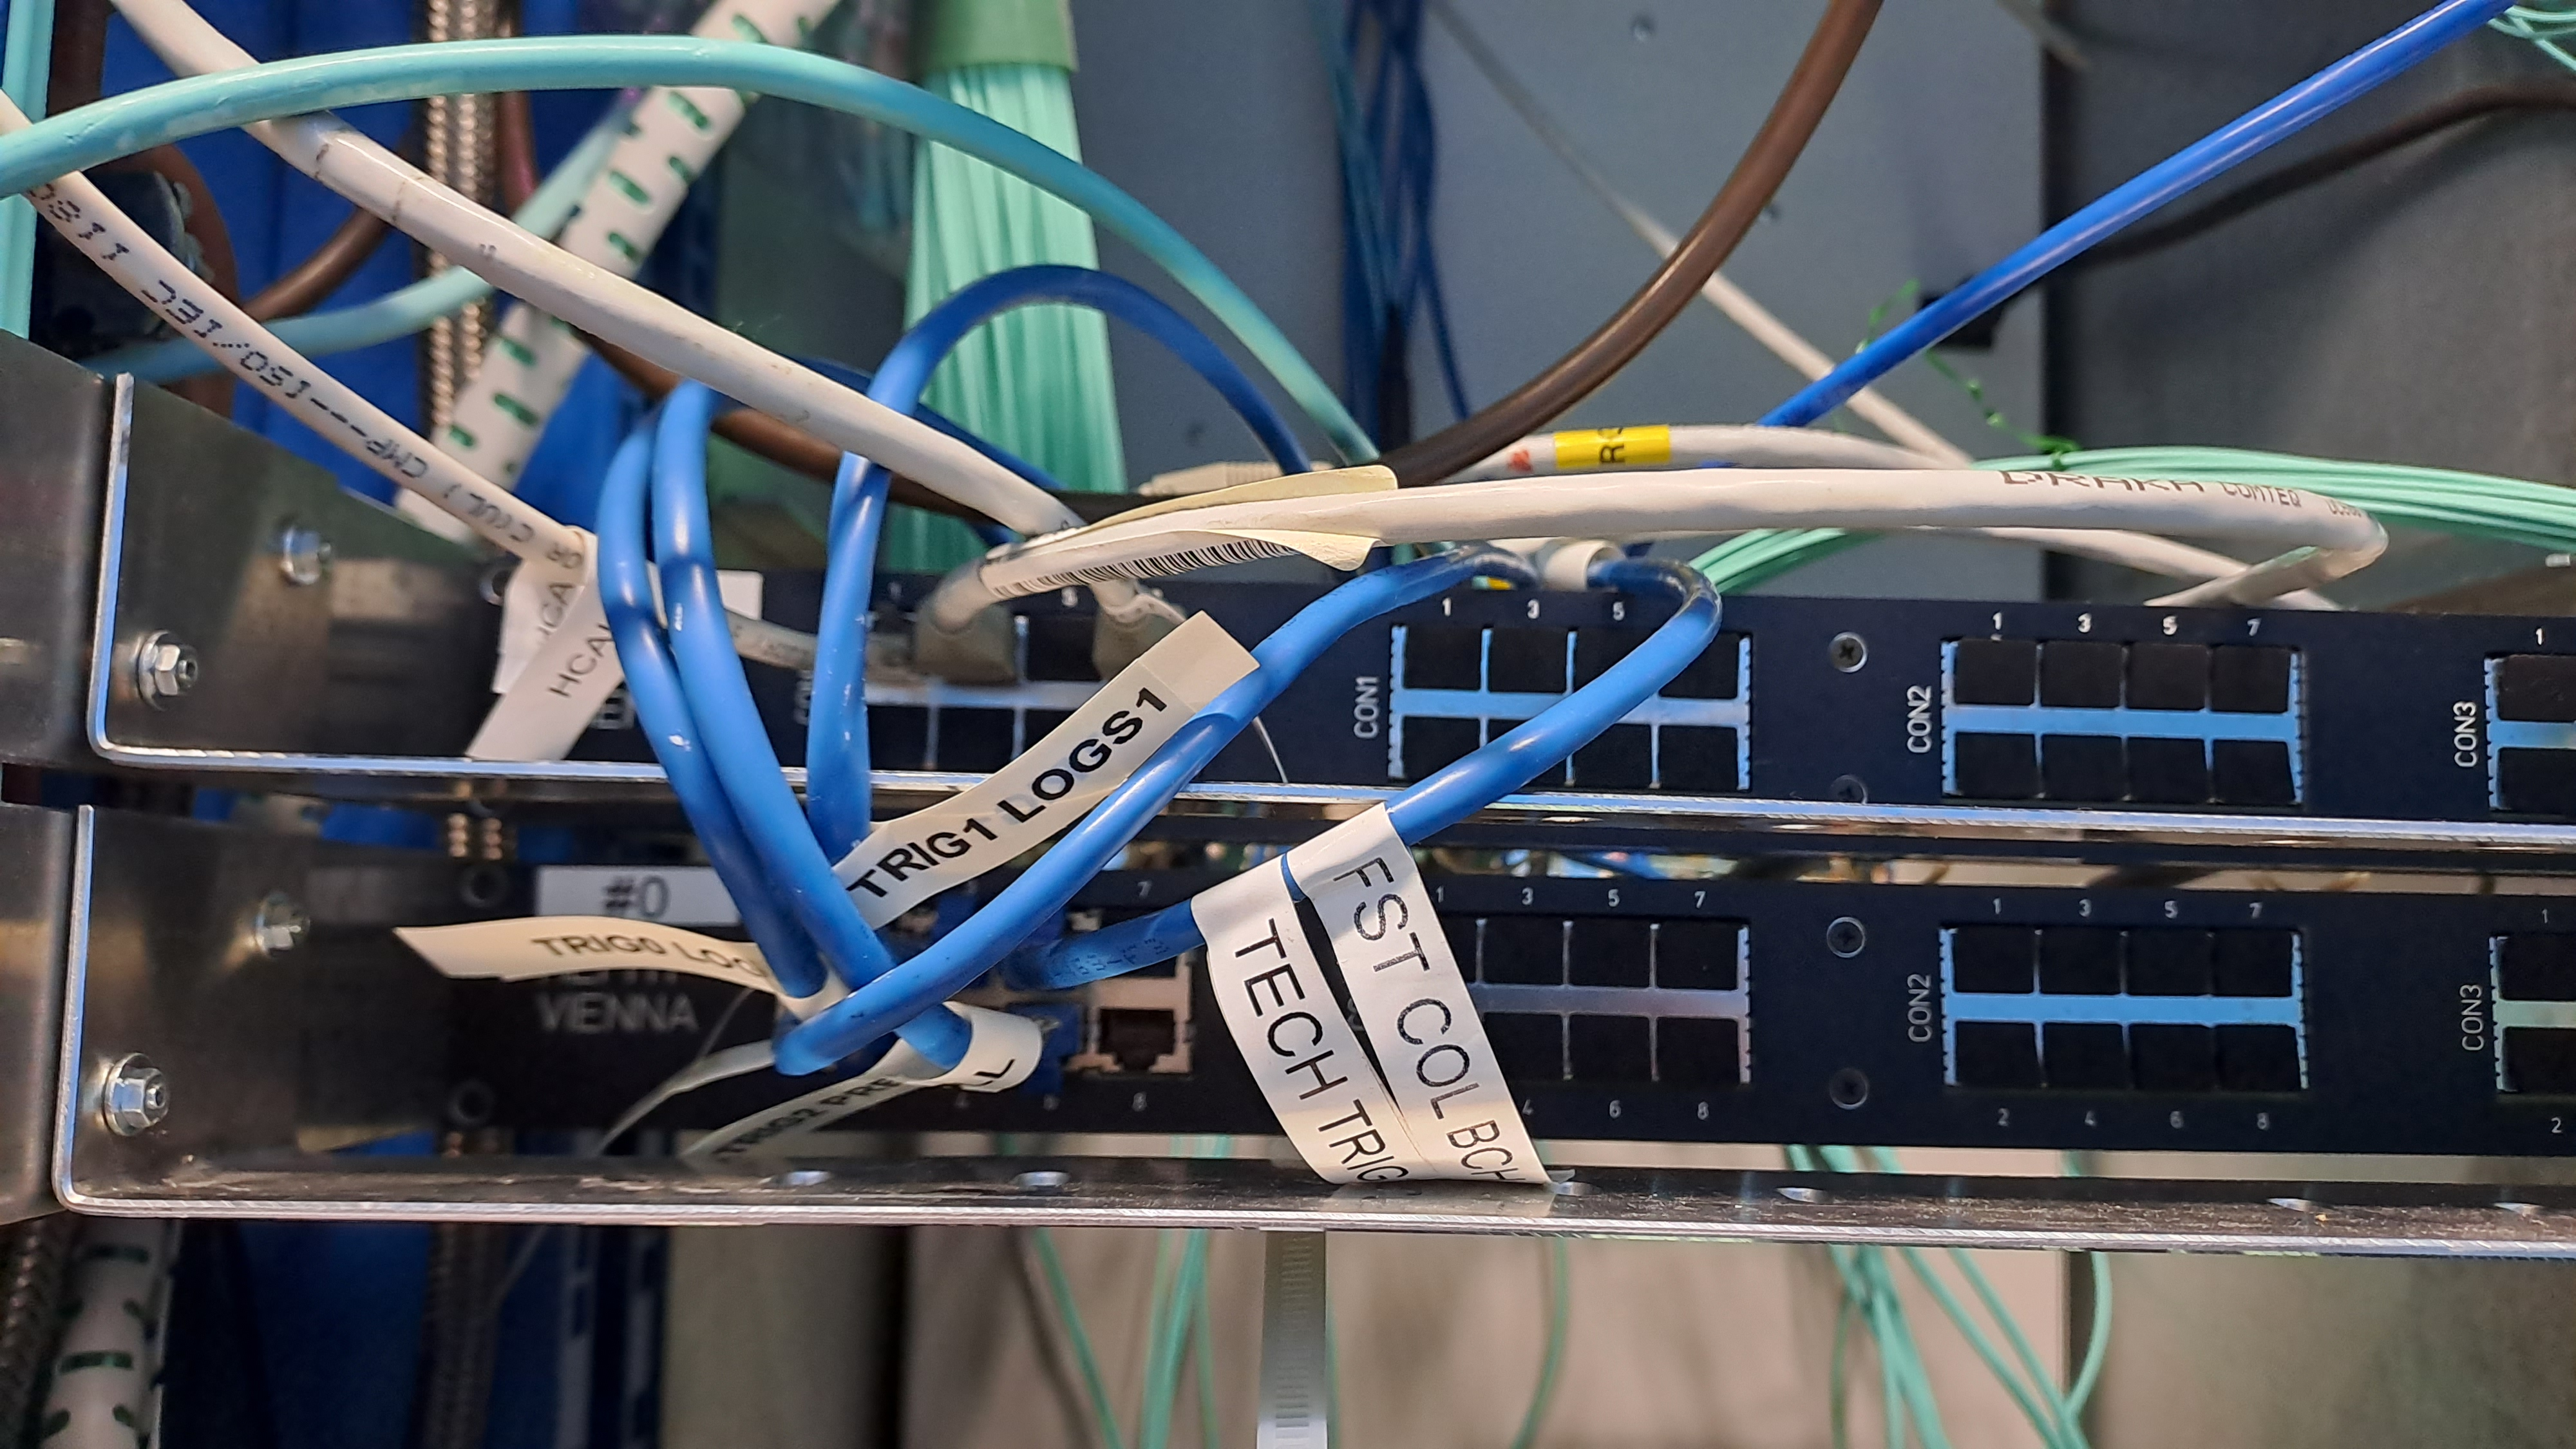
\includegraphics[width=15cm]{figures/ext_cond_pp}
\caption{External condtion patch panel (picture date: September 12, 2023)}
\label{fig:appl:ext_cond_pp}
\end{figure}

\clearpage

